\documentclass[border=12pt]{standalone}
\def\pgfsysdriver{pgfsys-dvisvgm.def}
\usepackage[dvisvgm]{xcolor}
\usepackage{xeCJK}
\setCJKmainfont{HaranoAjiGothic-Regular.otf}[BoldFont=HaranoAjiGothic-Bold.otf]
\setCJKsansfont{HaranoAjiGothic-Regular.otf}[BoldFont=HaranoAjiGothic-Bold.otf]
\usepackage{amsmath,amssymb,tikz,lmodern}
\usetikzlibrary{arrows.meta,positioning,calc,fit,backgrounds}
\renewcommand{\familydefault}{\sfdefault}
\definecolor{ink}{HTML}{25322F}
\definecolor{green}{HTML}{246657}
\definecolor{tint}{HTML}{EEF4F0}
\definecolor{soft}{HTML}{C6D2CC}
\definecolor{muted}{HTML}{52615B}
\newif\ifJapanese
\newcommand{\Tx}[2]{\ifJapanese #1\else #2\fi}
\newcommand{\Eff}{\overline{\operatorname{Eff}}}
\newcommand{\heading}[3]{{\color{green}\bfseries #1\quad\Tx{#2}{#3}}\\[5pt]}
% A white rectangle makes the complete citation label clickable, including spaces.
\newcommand{\refurl}[2]{\special{dvisvgm:raw <a xlink:href="#1" target="_blank" rel="noopener noreferrer">}{\setlength{\fboxsep}{0pt}\colorbox{white}{\color{green}\underline{\strut #2}}}\special{dvisvgm:raw </a>}}
\newcommand{\refedge}[3]{\refurl{\csname source#1\endcsname\string##page=#2}{#3}}
\newcommand{\SF}[2]{\refedge{sf}{#1}{#2}}
% GitHub's file preview does not support PDF page fragments.
\newcommand{\LA}[2]{\refurl{\sourcela}{#2}}
\newcommand{\Sch}[2]{\refedge{sch}{#1}{#2}}
\newcommand{\PS}[2]{\refedge{ps}{#1}{#2}}
\tikzset{
 card/.style={draw=soft,fill=white,rounded corners=2pt,align=left,text=ink,font=\fontsize{10.5}{14}\selectfont,inner xsep=12pt,inner ysep=10pt,text width=14.4cm},
 half/.style={card,text width=6.45cm,minimum height=2.05cm},
 result/.style={card,draw=green,fill=tint,line width=.9pt},
 reason/.style={align=left,text=muted,font=\fontsize{9}{12}\selectfont,inner sep=0pt,text width=12.7cm},
 branchreason/.style={reason,text width=5.95cm},
 edge/.style={-{Stealth[length=2.4mm]},draw=green,line width=1pt},
 wire/.style={draw=green,line width=1pt},
}
% Keep the arrow in a dedicated left gutter; explanations never cover it.
\newcommand{\flow}[3]{
 \coordinate (#2-from) at ($(#1.south)+(-6.9,0)$);
 \coordinate (#2-to) at ($(#2.north)+(-6.9,0)$);
 \draw[edge] (#2-from)--(#2-to);
 \node[reason,anchor=west] (#2-reason) at ($(#2-from)!.5!(#2-to)+(.55,0)$) {#3};
}

\newcommand{\Hash}[2]{\refurl{\sourcehash}{#2}}
\newcommand{\FGring}[2]{\refedge{rings}{#1}{#2}}
\newcommand{\FGglue}[2]{\refedge{glue}{#1}{#2}}
\newcommand{\OI}[2]{\refurl{\sourceoi}{#2}}

\Japanesefalse
\newcommand{\sourcela}{https://github.com/openai/math/blob/adc7f1241b42e322a6451854ab7e4b4c146bf78a/preprints/Log-abundance-in-characteristic-zero-September-24-2026/paper.pdf}
\newcommand{\sourcehash}{https://arxiv.org/html/1609.00121v4}
\newcommand{\sourceglue}{https://www.math.kyoto-u.ac.jp/~fujino/fg-comp-final.pdf}
\newcommand{\sourcerings}{https://www.math.kyoto-u.ac.jp/~fujino/log-ring-aspm.pdf}
\newcommand{\sourceoi}{https://github.com/openai/math/blob/adc7f1241b42e322a6451854ab7e4b4c146bf78a/preprints/Orbifold-and-logarithmic-Iitaka-subadditivity-September-26-2026/paper.pdf}
\newcommand{\sourcehps}{https://people.math.harvard.edu/~mpopa/papers/HPS.pdf}
\newcommand{\sourcegmm}{https://github.com/openai/math/blob/adc7f1241b42e322a6451854ab7e4b4c146bf78a/preprints/Minimal-models-and-Mori-fibre-spaces-for-generalized-log-canonical-Q-pairs-September-24-2026/paper.pdf}
\begin{document}
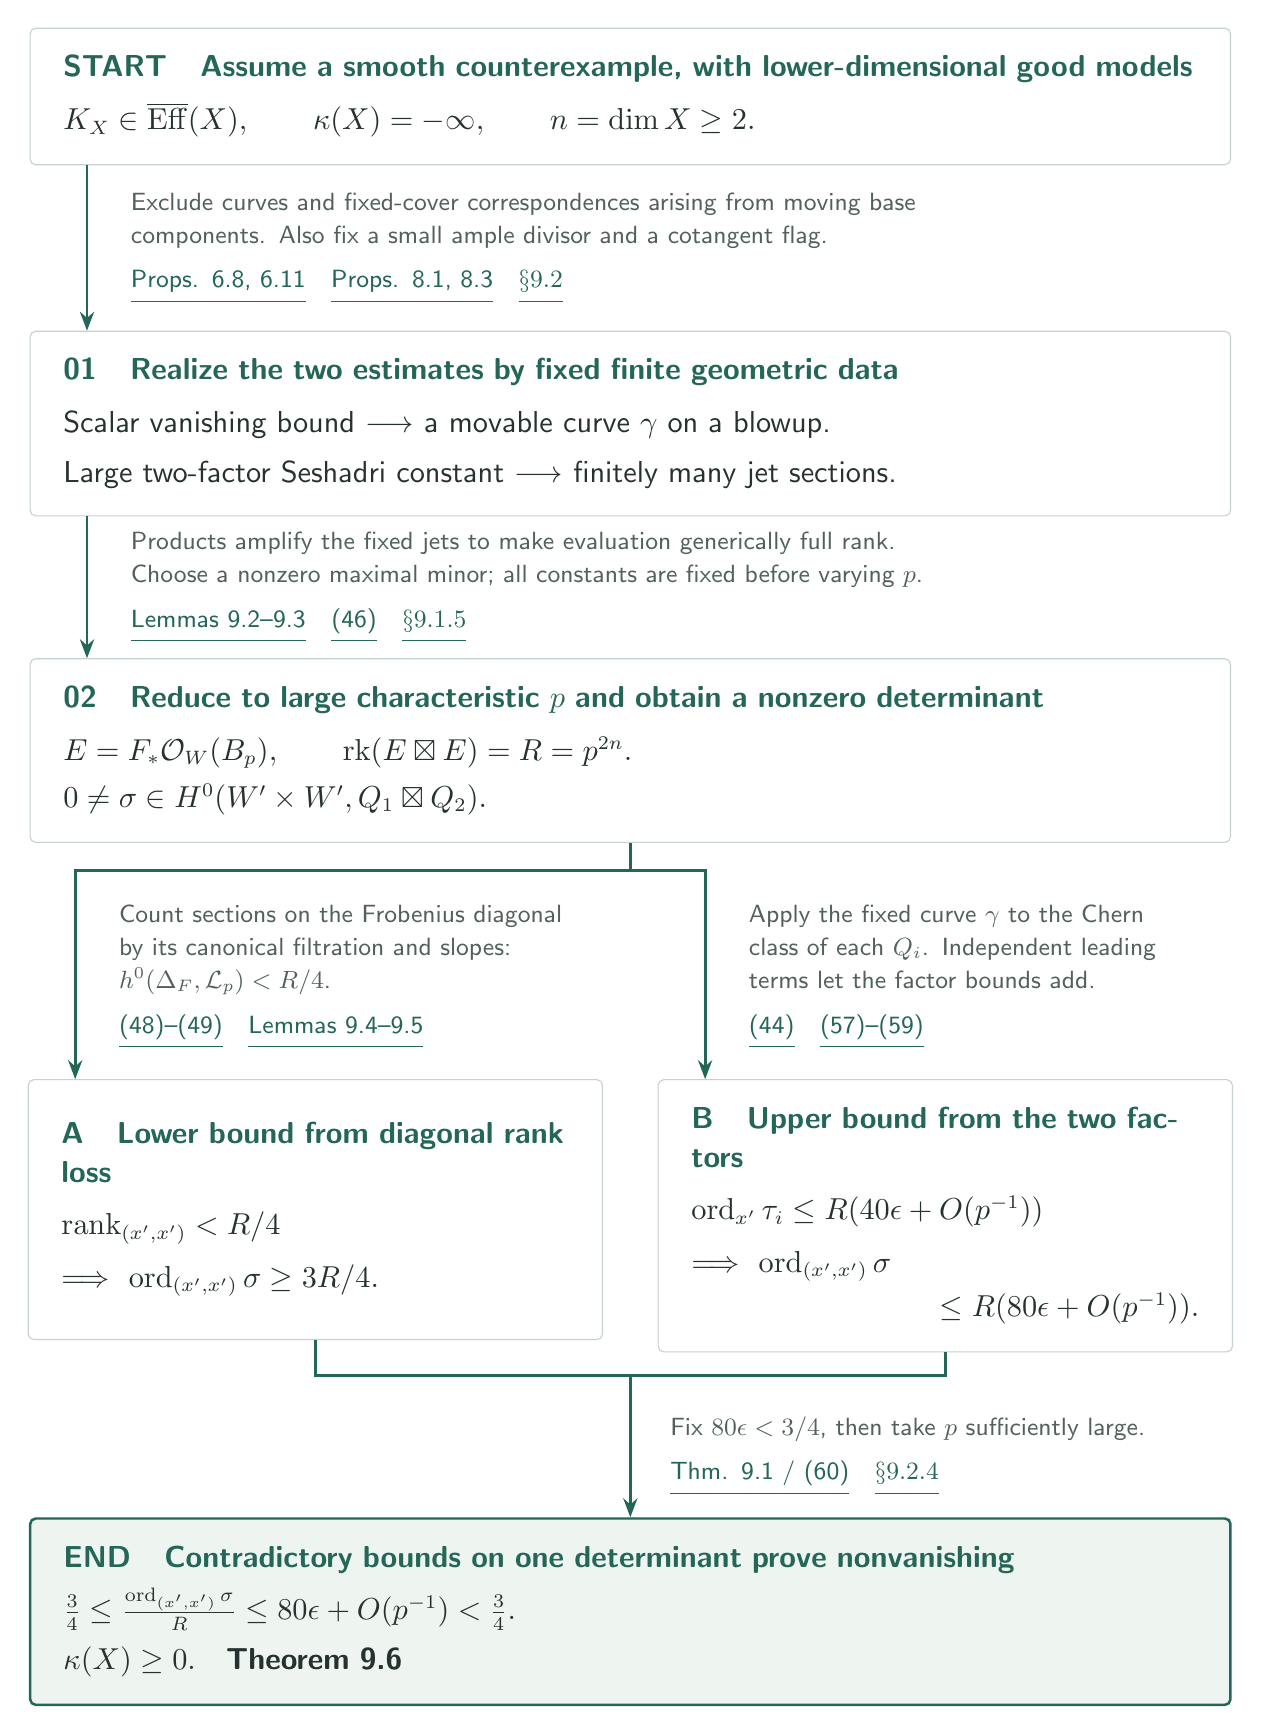
\begin{tikzpicture}
\node[card] (start) {\heading{START}{低次元の良いモデルの下で、滑らかな反例を仮定する}{Assume a smooth counterexample, with lower-dimensional good models}
$K_X\in\Eff(X),\qquad\kappa(X)=-\infty,\qquad n=\dim X\geq2.$};
\node[card,below=2.1cm of start] (witness) {\heading{01}{二種類の評価を、有限個の幾何データにする}{Realize the two estimates by fixed finite geometric data}
\Tx{スカラー切断の消滅上界 $\longrightarrow$ 爆発上の可動曲線 $\gamma$。}{Scalar vanishing bound $\longrightarrow$ a movable curve $\gamma$ on a blowup.}\\[4pt]
\Tx{二因子上の大きな Seshadri 定数 $\longrightarrow$ 有限個のジェット切断。}{Large two-factor Seshadri constant $\longrightarrow$ finitely many jet sections.}};
\flow{start}{witness}{\Tx{動く基底成分から生じる曲線族・固定被覆間の対応を排除。\\小さい豊富因子と余接束の旗も固定する。}{Exclude curves and fixed-cover correspondences arising from moving base\\components. Also fix a small ample divisor and a cotangent flag.}\\[4pt]\LA{38}{Props. 6.8, 6.11}\quad\LA{53}{Props. 8.1, 8.3}\quad\LA{69}{$\S9.2$}}
\node[card,below=1.8cm of witness] (matrix) {\heading{02}{大きい標数 $p$ へ還元し、非零の行列式を得る}{Reduce to large characteristic $p$ and obtain a nonzero determinant}
$E=F_*\mathcal O_W(B_p),\qquad \operatorname{rk}(E\boxtimes E)=R=p^{2n}.$\\[3pt]
$0\neq\sigma\in H^0(W'\times W',Q_1\boxtimes Q_2).$};
\flow{witness}{matrix}{\Tx{固定したジェットを積で増幅し、評価写像を一般点で full rank にする。\\その最大小行列式を一つ選ぶ。全ての定数は $p$ より先に固定。}{Products amplify the fixed jets to make evaluation generically full rank.\\Choose a nonzero maximal minor; all constants are fixed before varying $p$.}\\[4pt]\LA{63}{Lemmas 9.2--9.3}\quad\LA{64}{(46)}\quad\LA{67}{$\S9.1.5$}}
\node[half,below=3cm of matrix.south,anchor=north,xshift=-4cm,minimum height=3.3cm] (lower) {\heading{A}{対角上のランク欠損から下界}{Lower bound from diagonal rank loss}
$\operatorname{rank}_{(x',x')}<R/4$\\[5pt]
$\Longrightarrow\ \operatorname{ord}_{(x',x')}\sigma\geq3R/4.$};
\node[half,below=3cm of matrix.south,anchor=north,xshift=4cm,minimum height=3.3cm] (upper) {\heading{B}{二つの因子の次数から上界}{Upper bound from the two factors}
$\operatorname{ord}_{x'}\tau_i\leq R(40\epsilon+O(p^{-1}))$\\[5pt]
$\Longrightarrow\ \operatorname{ord}_{(x',x')}\sigma$\\[2pt]
$\hfill\leq R(80\epsilon+O(p^{-1})).$};
\draw[wire] (matrix.south)--++(0,-.35) coordinate (fork);
\draw[edge] (fork)-| ($(lower.north)+(-3.05,0)$);
\draw[edge] (fork)-| ($(upper.north)+(-3.05,0)$);
\node[branchreason,anchor=west] at ($(lower.north)+(-2.5,1.3)$) {\Tx{Frobenius 対角の切断を\\標準フィルトレーションと傾きで数え、\\$h^0(\Delta_F,\mathcal L_p)<R/4$ を得る。}{Count sections on the Frobenius diagonal\\by its canonical filtration and slopes:\\$h^0(\Delta_F,\mathcal L_p)<R/4$.}\\[4pt]\LA{65}{(48)--(49)}\quad\LA{66}{Lemmas 9.4--9.5}};
\node[branchreason,anchor=west] at ($(upper.north)+(-2.5,1.3)$) {\Tx{各 $Q_i$ の Chern 類に\\固定した曲線 $\gamma$ の評価を適用。\\先頭項の独立性で二因子の上界を足す。}{Apply the fixed curve $\gamma$ to the Chern\\class of each $Q_i$. Independent leading\\terms let the factor bounds add.}\\[4pt]\LA{62}{(44)}\quad\LA{68}{(57)--(59)}};
\node[result,below=2.25cm of lower.south,anchor=north,xshift=4cm] (end) {\heading{END}{同じ行列式の上下界が矛盾し、非消滅を得る}{Contradictory bounds on one determinant prove nonvanishing}
$\frac34\leq\frac{\operatorname{ord}_{(x',x')}\sigma}{R}\leq80\epsilon+O(p^{-1})<\frac34.$\\[4pt]
$\kappa(X)\geq0.$\quad\textbf{Theorem 9.6}};
\coordinate (join) at ($(end.north)+(0,1.8)$);
\draw[wire] (lower.south)|-(join);
\draw[wire] (upper.south)|-(join);
\draw[edge] (join)--(end.north);
\node[reason,text width=6.7cm,anchor=west] at ($(end.north)+(.5,.78)$) {\Tx{$80\epsilon<3/4$ を固定し、$p$ を十分大きくする。}{Fix $80\epsilon<3/4$, then take $p$ sufficiently large.}\\[4pt]\LA{69}{Thm. 9.1 / (60)}\quad\LA{72}{$\S9.2.4$}};
\end{tikzpicture}

\end{document}
